\documentclass{beamer}
\usepackage{multicol,lipsum,caption,graphicx}
\usepackage{mathtools, amsmath,booktabs,verbatim,tikz} 
\usetikzlibrary{shapes.geometric, arrows,positioning,matrix,calc}
%\usepackage{mathptmx}

\newcommand\scalemath[2]{\scalebox{#1}{\mbox{\ensuremath{\displaystyle #2}}}}

\usetheme[progressbar=frametitle]{metropolis}
\setbeamertemplate{frame numbering}[fraction]
\useoutertheme{metropolis}
\useinnertheme{metropolis}
\usefonttheme{metropolis}
\usecolortheme{spruce}
\setbeamercolor{background canvas}{bg=white}

\title{Optimum design of laminated composites for minimum thickness by a 
self-adaptative genetic algorithm}
\author{Huiyao Zhang}
\institute{Kyoto Institue of Technology}
\date{02-12-2020}
\setbeamertemplate{itemize/enumerate body begin}{\large}

\DeclarePairedDelimiter\Floor\lfloor\rfloor
\DeclarePairedDelimiter\Ceil\lceil\rceil
\begin{document}
\begin{frame}
    \titlepage
\end{frame}


\begin{frame}[c]{Content} 
    \begin{enumerate}
        \item Classic lamination theory
        \item Failure theory for composite material
        \item Self-adaptative genetic algorithm
        \item Experiment and result
        \item Comparison with related research
    \end{enumerate}
\end{frame}



\begin{frame}{1. Classic Lamination Theory}
    \begin{columns}[c]
    \begin{column}{0.5\textwidth}
        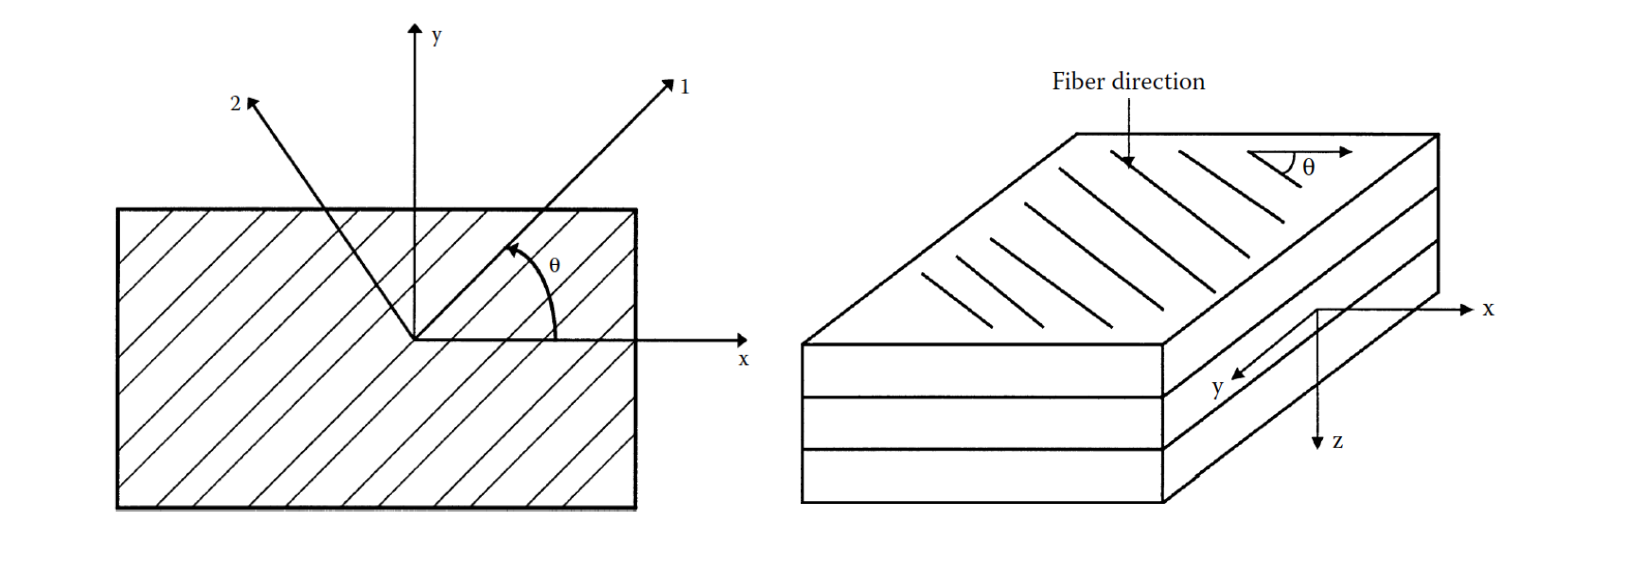
\includegraphics[width=1.5\linewidth]{../data/lamina_local_global_axes.png}
        \captionof{figure}{Composite Material}
    \end{column}
	\begin{column}{0.5\textwidth}
		\begin{equation} \label{eq:force_and_moments}
			\begin{array}{l}
				\begin{aligned}
			\begin{bmatrix}
				N_x \\
				N_y \\
				N_{xy}
			\end{bmatrix}
			&=
			\begin{bmatrix}
				A_{11} & A_{12} & A_{16} \\
				A_{12} & A_{22} & A_{26} \\
				A_{16} & A_{26} & A_{66} 
			\end{bmatrix}
			\begin{bmatrix}
				\varepsilon_x^0 \\
				\varepsilon_y^0 \\
				\gamma_{xy}^0
			\end{bmatrix}   \\
			&+               
			\begin{bmatrix}
				B_{11} & B_{12} & B_{16} \\
				B_{11} & B_{12} & B_{16} \\
				B_{16} & B_{26} & B_{66} 
			\end{bmatrix}
			\begin{bmatrix}
				k_x \\
				k_y \\
				k_{xy} 
			\end{bmatrix}  \\
		\end{aligned} \\ \\
		\begin{aligned}
			\begin{bmatrix}
				M_x \\
				M_y \\
				M_{xy}
			\end{bmatrix}
			&=
			\begin{bmatrix}
				B_{11} & B_{12} & B_{16} \\
				B_{12} & B_{22} & B_{26} \\
				B_{16} & B_{26} & B_{66} 
			\end{bmatrix}
			\begin{bmatrix}
				\varepsilon_x^0 \\
				\varepsilon_y^0 \\
				\gamma_{xy}^0
			\end{bmatrix} \\ 
			&+  
			\begin{bmatrix}
				D_{11} & D_{12} & D_{16} \\
				D_{11} & D_{12} & D_{16} \\
				D_{16} & D_{26} & D_{66} 
			\end{bmatrix}
			\begin{bmatrix}
				k_x \\
				k_y \\
				k_{xy} 
			\end{bmatrix}
		\end{aligned}
			\end{array}
		\end{equation}
	\end{column}
\end{columns}
\end{frame}

\begin{frame}{2. Failure Theory }
\begin{columns}[c]
    \begin{column}{0.4\textwidth}
		\begin{figure}
		\centering
		\resizebox{1.2\linewidth}{!}{
		\begin{tikzpicture}
			\begin{scope}
				%\draw[style=help lines] (-3,-3) grid (3,3);
				\draw (0,0) rectangle (2,3);
				\draw[->] (1.3,1.2) -- (2.6,1.2);
				\draw[->] (1.3,1.2) -- (1.3,3.4);
				\node at (2.2,1) {$X_T$};
				\node at (1.5, 3.2) {$Y_T$};
				\node at (-0.2, 0.9) {$X_C$};
				\node at (1.8, -0.2) {$Y_C$};
			\end{scope}
			\begin{scope}[xshift=6cm,yshift=1.15cm]
				%\draw[style=help lines] (-3,-3) grid (3,3);
				\draw[rotate=30] (0,0) ellipse (2cm and 1cm);
				\draw[->] (0.2,0) -- (0.2,2.2);
				\draw[->] (0.2,0) -- (1.9,0);
				\node at (1.6,-0.2) {$X_T$};
				\node at (0.3, 1.3) {$Y_T$};
				\node at (-1.6, 0) {$X_C$};
				\node at (-0.5, -1.5) {$Y_C$};
			\end{scope}
		\end{tikzpicture}
		}
		\caption{Schematic failure surfaces for maximum stress and quadratic failure
		criteria}
		\end{figure}
    \end{column}
    \begin{column}{0.6\textwidth}
		\begin{itemize}
			\item  Maximum stress failure
				\begingroup
				\small
				\begin{align*}
					SF_{MS}^k = \text{min of}
					\begin{cases}
						SF_X^k = 
						\begin{cases}
							\frac{X_t}{\sigma_{11}}, \text{ if } \sigma_{11}>0 \\
							\frac{X_c}{\sigma_{11}}, \text{ if } \sigma_{11}<0 \\
						\end{cases} \\
						SF_Y^k = 
						\begin{cases}
							\frac{Y_t}{\sigma_{22}}, \text{ if } \sigma_{22}>0 \\
							\frac{Y_c}{\sigma_{22}}, \text{ if } \sigma_{22}<0 \\
						\end{cases} \\
						SF_S^k =
						\begin{cases}
							\frac{S}{|\tau_{12}|} \\
						\end{cases} \\
					\end{cases} \textstyle{.}
				\end{align*}
				\endgroup
			\item  Tsai-wu failure theory

		 \begingroup
		 \small
		 \begin{equation*} 
		 \begin{split}
			H_1 \sigma_1  & + H_2 \sigma_2 + H_6 \tau_{12} + H_{11}\sigma_1^2 + H_{22} \sigma_2^2 \\
						  & + H_{66}  \tau_{12}^2 + 2H_{12}\sigma_1\sigma_2 < 1
		 \end{split}
		\end{equation*}
		\endgroup
		\end{itemize}
    \end{column}
\end{columns}
\end{frame}

\begin{frame}{3. Self-adaptative GA}
    \begin{columns}[c]
    \begin{column}{1\textwidth}
		\begin{itemize}
			\item Modifying selection strategy: in order to handle the constraint search
			\item Self-adaptative mutation direction of fiber orientation and laminate thickness:
				random change the length, and the angle in the laminate.
			\item The self-adaptative parameters don't refer to parent's proportion, mutation
				probability.
		\end{itemize}
    \end{column}
    \begin{column}{0.8\textwidth}

    \end{column}
\end{columns}
\end{frame}

\begin{frame}{3. Self-adaptative GA: selection operator}
    \begin{columns}[c]
    \begin{column}{0.8\textwidth}
		\begin{itemize}
			\item acitve group: individual is used to increase the diversity of the population
			\item potential group: individual doesn't fulfill constraint
			\item proper group: individual meet constraint
		\end{itemize}
		
    \end{column}
\end{columns}
\end{frame}

\begin{frame}{3. Self-adaptative GA:  mutation operator}
    \begin{columns}[c]
    \begin{column}{1\textwidth}
		$\text{md} = [CT_1, \cdots, CT_{n-1}, CT_n] -  [ICV_0, \cdots, ICV_{n-1},
		ICV_n]$ \\
		\begin{itemize}
			\item  md means mutation direction.
			\item  $CT_i$ denotes the i-th constraint, such as weight, safety factor.
			\item  $ICV_i$ denotes individual's i-th constraint value, such as,  weight, safety
				factor of current individual.
		\end{itemize}

    \end{column}
\end{columns}
\end{frame}


\begin{frame}{4. Self-adaptative GA:  mutation operator}
    \begin{columns}[c]
	\begin{column}{1\textwidth}
		\begin{itemize}
			\item length mutation =  
				\[
				  \begin{cases}
					  LMC*[0, \sum_{i=1}^{N}{md_i}] & \text{if $\sum_{i=1}^{N}{md_i} > 0$} \\
					  LMC*[\sum_{i=1}^{N}{md_i}, 0] & \text{if $\sum_{i=1}^{N}{md_i} < 0$} \\
				  \end{cases}
				\] \\
				LMC stands for length mutation coefficient, it's a positive integer.
			\item angle mutation = 
				\[
				  \begin{cases}
					  AMC*[0, \sum_{i=1}^{N}{md_i}] & \text{if $\sum_{i=1}^{N}{md_i} > 0$} \\
					  AMC*[\sum_{i=1}^{N}{md_i}, 0] & \text{if $\sum_{i=1}^{N}{md_i} < 0$} \\
				  \end{cases}
				\] \\
				AMC stands for angle mutation coefficient, it's sign is unclear.
		\end{itemize}
	\end{column}
\end{columns}
\end{frame}



\begin{frame}{5. Result: Loading $N_x = 10, N_y=5 $ MPa m}
    \begin{columns}
    \begin{column}{0.5\textwidth}

        \begin{center}
            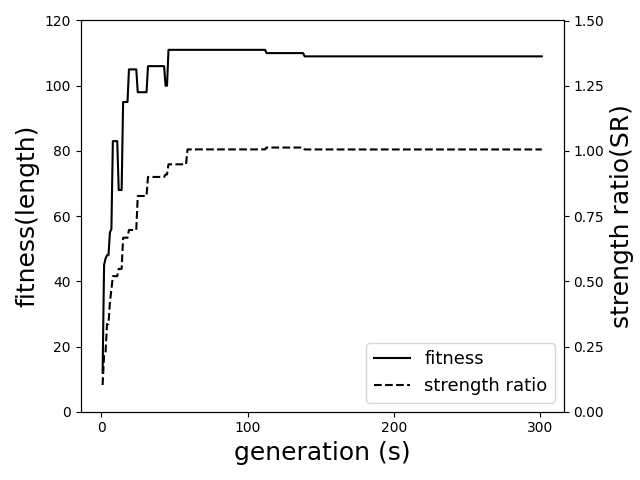
\includegraphics[width=1.0\linewidth]{2020-11-10-pre-image/two_distinct_angle_fitness_and_sr.png}
        \end{center}

        \begin{center}
              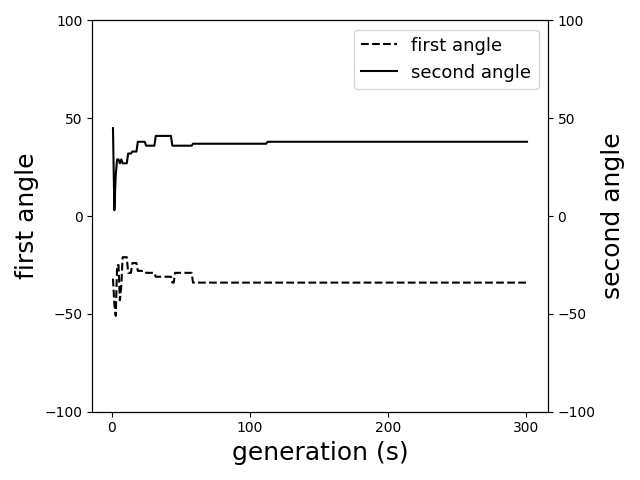
\includegraphics[width=1.0\linewidth]{2020-11-10-pre-image/two_distinct_angle_angle_change.png}
        \end{center}
    \end{column}
    \begin{column}{0.5\textwidth}
        \begin{center}
              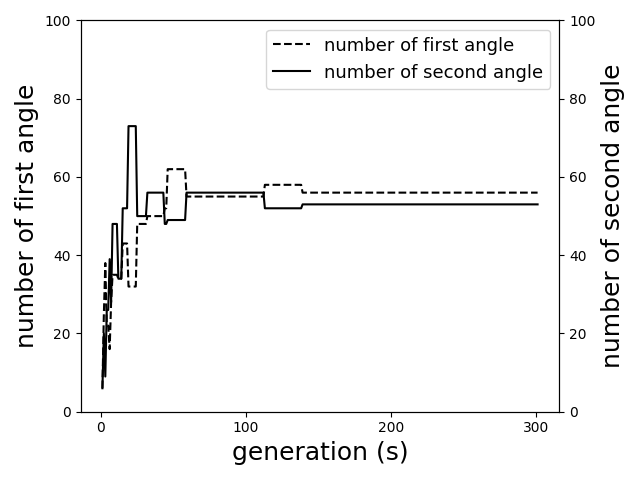
\includegraphics[width=1.0\linewidth]{2020-11-10-pre-image/two_distinct_angler_number_change.png}
              \captionof{figure}{Two distinct angles in the laminate}
        \end{center}
    \end{column}
\end{columns}
\end{frame}


\begin{frame}{6. Comparison with related research}

\begin{table}
	\normalsize
\caption{Comparison with the results of DSA}
\label{tab:comparision}
\centering
	\resizebox{10cm}{!}{
\begin{tabular}{c|cccc|lccc}
	\toprule
	\textbf{Loading}	    & \multicolumn {4}{c}{\textbf{Akbulut and Sonmez's Study}}   & \multicolumn {4}{c}{\textbf{Present Study}}\\
	\midrule
	 $N_{x}/N_{y}/N_{xy}$   & Optimum lay-up			        & laminate  & TW & MS   & Optimum lay-up & laminate  & TW & MS \\
	  (MPa m)	            & sequences					        & thickness &    &      & sequences	     & thickness &    &    \\
	\midrule
	  10/5/0                 &  $[37_{27}/\text{-}37_{27}]_s$     &  108      &  1.0068  &  1.0277 & $[33_{29}/\text{-}39_{25}/\bar{\text{-}39}]_s$     &     109      &  1.0074      &  1.0246  \\
	  20/5/0                 &  $[31_{23}/\text{-}31_{23}]_s$     &  92       &  1.0208  &  1.1985 & $[33_{22}/\text{-}31_{24}]_s$                      &     92      &  1.0055       &  1.2065    \\
	  40/5/0                 &  $[26_{20}/\text{-}26_{20}]_s$     &  80       &  1.0190  &  1.5381 & $[29_{18}/\text{-}21_{23}/\bar{\text{-}21}]_s$     &     83      &  1.0034       &  1.7350   \\
	  80/5/0                 &  $[21_{25}/\text{-}19_{28}]_s$     &  106      &  1.0113  &  1.2213 & $[\text{-}20_{27}/21_{25}/\bar{25}]_s$             &     105      &  1.0029      &  1.2063    \\
	  120/5/0                &  $[17_{35}/\text{-}17_{35}]_s$     &  140      &  1.0030  &  1.0950 & $[\text{-}18_{34}/17_{36}]_s$                     &     140      &  1.0000      &  1.0898     \\
	\bottomrule
\end{tabular}
}
\end{table}
\end{frame}



\end{document}
